% Options for packages loaded elsewhere
\PassOptionsToPackage{unicode}{hyperref}
\PassOptionsToPackage{hyphens}{url}
%
\documentclass[
]{article}
\usepackage{amsmath,amssymb}
\usepackage{iftex}
\ifPDFTeX
  \usepackage[T1]{fontenc}
  \usepackage[utf8]{inputenc}
  \usepackage{textcomp} % provide euro and other symbols
\else % if luatex or xetex
  \usepackage{unicode-math} % this also loads fontspec
  \defaultfontfeatures{Scale=MatchLowercase}
  \defaultfontfeatures[\rmfamily]{Ligatures=TeX,Scale=1}
\fi
\usepackage{lmodern}
\ifPDFTeX\else
  % xetex/luatex font selection
\fi
% Use upquote if available, for straight quotes in verbatim environments
\IfFileExists{upquote.sty}{\usepackage{upquote}}{}
\IfFileExists{microtype.sty}{% use microtype if available
  \usepackage[]{microtype}
  \UseMicrotypeSet[protrusion]{basicmath} % disable protrusion for tt fonts
}{}
\makeatletter
\@ifundefined{KOMAClassName}{% if non-KOMA class
  \IfFileExists{parskip.sty}{%
    \usepackage{parskip}
  }{% else
    \setlength{\parindent}{0pt}
    \setlength{\parskip}{6pt plus 2pt minus 1pt}}
}{% if KOMA class
  \KOMAoptions{parskip=half}}
\makeatother
\usepackage{xcolor}
\usepackage[margin=1in]{geometry}
\usepackage{color}
\usepackage{fancyvrb}
\newcommand{\VerbBar}{|}
\newcommand{\VERB}{\Verb[commandchars=\\\{\}]}
\DefineVerbatimEnvironment{Highlighting}{Verbatim}{commandchars=\\\{\}}
% Add ',fontsize=\small' for more characters per line
\usepackage{framed}
\definecolor{shadecolor}{RGB}{248,248,248}
\newenvironment{Shaded}{\begin{snugshade}}{\end{snugshade}}
\newcommand{\AlertTok}[1]{\textcolor[rgb]{0.94,0.16,0.16}{#1}}
\newcommand{\AnnotationTok}[1]{\textcolor[rgb]{0.56,0.35,0.01}{\textbf{\textit{#1}}}}
\newcommand{\AttributeTok}[1]{\textcolor[rgb]{0.13,0.29,0.53}{#1}}
\newcommand{\BaseNTok}[1]{\textcolor[rgb]{0.00,0.00,0.81}{#1}}
\newcommand{\BuiltInTok}[1]{#1}
\newcommand{\CharTok}[1]{\textcolor[rgb]{0.31,0.60,0.02}{#1}}
\newcommand{\CommentTok}[1]{\textcolor[rgb]{0.56,0.35,0.01}{\textit{#1}}}
\newcommand{\CommentVarTok}[1]{\textcolor[rgb]{0.56,0.35,0.01}{\textbf{\textit{#1}}}}
\newcommand{\ConstantTok}[1]{\textcolor[rgb]{0.56,0.35,0.01}{#1}}
\newcommand{\ControlFlowTok}[1]{\textcolor[rgb]{0.13,0.29,0.53}{\textbf{#1}}}
\newcommand{\DataTypeTok}[1]{\textcolor[rgb]{0.13,0.29,0.53}{#1}}
\newcommand{\DecValTok}[1]{\textcolor[rgb]{0.00,0.00,0.81}{#1}}
\newcommand{\DocumentationTok}[1]{\textcolor[rgb]{0.56,0.35,0.01}{\textbf{\textit{#1}}}}
\newcommand{\ErrorTok}[1]{\textcolor[rgb]{0.64,0.00,0.00}{\textbf{#1}}}
\newcommand{\ExtensionTok}[1]{#1}
\newcommand{\FloatTok}[1]{\textcolor[rgb]{0.00,0.00,0.81}{#1}}
\newcommand{\FunctionTok}[1]{\textcolor[rgb]{0.13,0.29,0.53}{\textbf{#1}}}
\newcommand{\ImportTok}[1]{#1}
\newcommand{\InformationTok}[1]{\textcolor[rgb]{0.56,0.35,0.01}{\textbf{\textit{#1}}}}
\newcommand{\KeywordTok}[1]{\textcolor[rgb]{0.13,0.29,0.53}{\textbf{#1}}}
\newcommand{\NormalTok}[1]{#1}
\newcommand{\OperatorTok}[1]{\textcolor[rgb]{0.81,0.36,0.00}{\textbf{#1}}}
\newcommand{\OtherTok}[1]{\textcolor[rgb]{0.56,0.35,0.01}{#1}}
\newcommand{\PreprocessorTok}[1]{\textcolor[rgb]{0.56,0.35,0.01}{\textit{#1}}}
\newcommand{\RegionMarkerTok}[1]{#1}
\newcommand{\SpecialCharTok}[1]{\textcolor[rgb]{0.81,0.36,0.00}{\textbf{#1}}}
\newcommand{\SpecialStringTok}[1]{\textcolor[rgb]{0.31,0.60,0.02}{#1}}
\newcommand{\StringTok}[1]{\textcolor[rgb]{0.31,0.60,0.02}{#1}}
\newcommand{\VariableTok}[1]{\textcolor[rgb]{0.00,0.00,0.00}{#1}}
\newcommand{\VerbatimStringTok}[1]{\textcolor[rgb]{0.31,0.60,0.02}{#1}}
\newcommand{\WarningTok}[1]{\textcolor[rgb]{0.56,0.35,0.01}{\textbf{\textit{#1}}}}
\usepackage{longtable,booktabs,array}
\usepackage{calc} % for calculating minipage widths
% Correct order of tables after \paragraph or \subparagraph
\usepackage{etoolbox}
\makeatletter
\patchcmd\longtable{\par}{\if@noskipsec\mbox{}\fi\par}{}{}
\makeatother
% Allow footnotes in longtable head/foot
\IfFileExists{footnotehyper.sty}{\usepackage{footnotehyper}}{\usepackage{footnote}}
\makesavenoteenv{longtable}
\usepackage{graphicx}
\makeatletter
\def\maxwidth{\ifdim\Gin@nat@width>\linewidth\linewidth\else\Gin@nat@width\fi}
\def\maxheight{\ifdim\Gin@nat@height>\textheight\textheight\else\Gin@nat@height\fi}
\makeatother
% Scale images if necessary, so that they will not overflow the page
% margins by default, and it is still possible to overwrite the defaults
% using explicit options in \includegraphics[width, height, ...]{}
\setkeys{Gin}{width=\maxwidth,height=\maxheight,keepaspectratio}
% Set default figure placement to htbp
\makeatletter
\def\fps@figure{htbp}
\makeatother
\setlength{\emergencystretch}{3em} % prevent overfull lines
\providecommand{\tightlist}{%
  \setlength{\itemsep}{0pt}\setlength{\parskip}{0pt}}
\setcounter{secnumdepth}{-\maxdimen} % remove section numbering
\ifLuaTeX
  \usepackage{selnolig}  % disable illegal ligatures
\fi
\IfFileExists{bookmark.sty}{\usepackage{bookmark}}{\usepackage{hyperref}}
\IfFileExists{xurl.sty}{\usepackage{xurl}}{} % add URL line breaks if available
\urlstyle{same}
\hypersetup{
  pdftitle={RNA Analysis 23},
  pdfauthor={Michael Callahan},
  hidelinks,
  pdfcreator={LaTeX via pandoc}}

\title{RNA Analysis 23}
\author{Michael Callahan}
\date{2024-04-03}

\begin{document}
\maketitle

\hypertarget{load-data}{%
\subsection{Load data}\label{load-data}}

\begin{Shaded}
\begin{Highlighting}[]
\FunctionTok{library}\NormalTok{(here)}
\end{Highlighting}
\end{Shaded}

\begin{verbatim}
## Warning: package 'here' was built under R version 4.3.3
\end{verbatim}

\begin{verbatim}
## here() starts at C:/Users/mgcal/OneDrive/Documents/School/Courses/Stat 555/Project/Stat555Project
\end{verbatim}

\begin{Shaded}
\begin{Highlighting}[]
\FunctionTok{library}\NormalTok{(dplyr)}
\end{Highlighting}
\end{Shaded}

\begin{verbatim}
## 
## Attaching package: 'dplyr'
\end{verbatim}

\begin{verbatim}
## The following objects are masked from 'package:stats':
## 
##     filter, lag
\end{verbatim}

\begin{verbatim}
## The following objects are masked from 'package:base':
## 
##     intersect, setdiff, setequal, union
\end{verbatim}

\begin{Shaded}
\begin{Highlighting}[]
\NormalTok{current\_project\_path }\OtherTok{\textless{}{-}} \FunctionTok{here}\NormalTok{()}

\NormalTok{file\_path }\OtherTok{\textless{}{-}} \FunctionTok{file.path}\NormalTok{(current\_project\_path, }\StringTok{"Data"}\NormalTok{, }\StringTok{"CMP\_RNA\_1.tsv"}\NormalTok{)}
\NormalTok{CMP\_RNA\_1 }\OtherTok{\textless{}{-}} \FunctionTok{read.delim}\NormalTok{(file\_path)}

\NormalTok{file\_path }\OtherTok{\textless{}{-}} \FunctionTok{file.path}\NormalTok{(current\_project\_path, }\StringTok{"Data"}\NormalTok{, }\StringTok{"CMP\_RNA\_2.tsv"}\NormalTok{)}
\NormalTok{CMP\_RNA\_2 }\OtherTok{\textless{}{-}} \FunctionTok{read.delim}\NormalTok{(file\_path)}

\NormalTok{file\_path }\OtherTok{\textless{}{-}} \FunctionTok{file.path}\NormalTok{(current\_project\_path, }\StringTok{"Data"}\NormalTok{, }\StringTok{"CFU{-}E\_RNA\_1.tsv"}\NormalTok{)}
\NormalTok{CFUE\_RNA\_1 }\OtherTok{\textless{}{-}} \FunctionTok{read.delim}\NormalTok{(file\_path)}

\NormalTok{file\_path }\OtherTok{\textless{}{-}} \FunctionTok{file.path}\NormalTok{(current\_project\_path, }\StringTok{"Data"}\NormalTok{, }\StringTok{"CFU{-}E\_RNA\_2.tsv"}\NormalTok{)}
\NormalTok{CFUE\_RNA\_2 }\OtherTok{\textless{}{-}} \FunctionTok{read.delim}\NormalTok{(file\_path)}
\end{Highlighting}
\end{Shaded}

\hypertarget{data-preprocessing}{%
\subsection{Data preprocessing}\label{data-preprocessing}}

\begin{Shaded}
\begin{Highlighting}[]
\CommentTok{\#FYI {-} gene\_ids are unique}

\CommentTok{\#CREATE A TPM Dataframe}
\CommentTok{\# Add prefixes to the tpm columns in each dataframe}
\NormalTok{CFUE\_RNA\_1\_tpm }\OtherTok{\textless{}{-}}\NormalTok{ CFUE\_RNA\_1 }\SpecialCharTok{\%\textgreater{}\%} \FunctionTok{select}\NormalTok{(gene\_id, }\AttributeTok{CFUE\_RNA\_1\_tpm =}\NormalTok{ TPM)}
\NormalTok{CFUE\_RNA\_2\_tpm }\OtherTok{\textless{}{-}}\NormalTok{ CFUE\_RNA\_2 }\SpecialCharTok{\%\textgreater{}\%} \FunctionTok{select}\NormalTok{(gene\_id, }\AttributeTok{CFUE\_RNA\_2\_tpm =}\NormalTok{ TPM)}
\NormalTok{CMP\_RNA\_1\_tpm }\OtherTok{\textless{}{-}}\NormalTok{ CMP\_RNA\_1 }\SpecialCharTok{\%\textgreater{}\%} \FunctionTok{select}\NormalTok{(gene\_id, }\AttributeTok{CMP\_RNA\_1\_tpm =}\NormalTok{ TPM)}
\NormalTok{CMP\_RNA\_2\_tpm }\OtherTok{\textless{}{-}}\NormalTok{ CMP\_RNA\_2 }\SpecialCharTok{\%\textgreater{}\%} \FunctionTok{select}\NormalTok{(gene\_id, }\AttributeTok{CMP\_RNA\_2\_tpm =}\NormalTok{ TPM)}

\CommentTok{\# Join the dataframes together on gene\_id}
\NormalTok{tpm }\OtherTok{\textless{}{-}} \FunctionTok{inner\_join}\NormalTok{(CFUE\_RNA\_1\_tpm, CFUE\_RNA\_2\_tpm, }\AttributeTok{by =} \StringTok{"gene\_id"}\NormalTok{) }\SpecialCharTok{\%\textgreater{}\%}
       \FunctionTok{inner\_join}\NormalTok{(CMP\_RNA\_1\_tpm, }\AttributeTok{by =} \StringTok{"gene\_id"}\NormalTok{) }\SpecialCharTok{\%\textgreater{}\%}
       \FunctionTok{inner\_join}\NormalTok{(CMP\_RNA\_2\_tpm, }\AttributeTok{by =} \StringTok{"gene\_id"}\NormalTok{) }

\FunctionTok{rm}\NormalTok{(CFUE\_RNA\_1\_tpm, CFUE\_RNA\_2\_tpm, CMP\_RNA\_1\_tpm, CMP\_RNA\_2\_tpm)}

\NormalTok{tpm }\OtherTok{\textless{}{-}}\NormalTok{ tpm }\SpecialCharTok{\%\textgreater{}\%}
  \FunctionTok{rename\_at}\NormalTok{(}\FunctionTok{vars}\NormalTok{(}\DecValTok{2}\SpecialCharTok{:}\DecValTok{5}\NormalTok{), }\SpecialCharTok{\textasciitilde{}} \FunctionTok{sub}\NormalTok{(}\StringTok{"\_tpm$"}\NormalTok{, }\StringTok{""}\NormalTok{, .))}


\CommentTok{\# Set \textquotesingle{}column\_name\textquotesingle{} as row names}
\FunctionTok{rownames}\NormalTok{(tpm) }\OtherTok{\textless{}{-}}\NormalTok{ tpm}\SpecialCharTok{$}\NormalTok{gene\_id}

\CommentTok{\# Remove \textquotesingle{}column\_name\textquotesingle{} from dataframe (optional)}
\NormalTok{tpm }\OtherTok{\textless{}{-}}\NormalTok{ tpm[, }\SpecialCharTok{{-}}\FunctionTok{which}\NormalTok{(}\FunctionTok{names}\NormalTok{(tpm) }\SpecialCharTok{==} \StringTok{\textquotesingle{}gene\_id\textquotesingle{}}\NormalTok{)]}

\CommentTok{\#Create a colData matrix}
\NormalTok{colData }\OtherTok{=} \FunctionTok{data.frame}\NormalTok{(}
  \AttributeTok{source\_name =} \FunctionTok{c}\NormalTok{(}\StringTok{\textquotesingle{}CMP\_RNA\_1\textquotesingle{}}\NormalTok{,}\StringTok{\textquotesingle{}CMP\_RNA\_2\textquotesingle{}}\NormalTok{,}\StringTok{\textquotesingle{}CFUE\_RNA\_1\textquotesingle{}}\NormalTok{,}\StringTok{\textquotesingle{}CFUE\_RNA\_2\textquotesingle{}}\NormalTok{),}
  \AttributeTok{group =} \FunctionTok{c}\NormalTok{(}\StringTok{\textquotesingle{}CMP\textquotesingle{}}\NormalTok{, }\StringTok{\textquotesingle{}CMP\textquotesingle{}}\NormalTok{, }\StringTok{\textquotesingle{}CFUE\textquotesingle{}}\NormalTok{, }\StringTok{\textquotesingle{}CFUE\textquotesingle{}}\NormalTok{)}
\NormalTok{  )}
\end{Highlighting}
\end{Shaded}

\hypertarget{histogram-overlay}{%
\subsection{Histogram overlay}\label{histogram-overlay}}

Here, we can see a density plot of the 4 samples being compared.

\begin{Shaded}
\begin{Highlighting}[]
\FunctionTok{library}\NormalTok{(RColorBrewer)}
\NormalTok{tpm\_filtered }\OtherTok{\textless{}{-}}\NormalTok{ tpm[}\FunctionTok{rowSums}\NormalTok{(tpm }\SpecialCharTok{!=} \DecValTok{0}\NormalTok{) }\SpecialCharTok{\textgreater{}} \DecValTok{0}\NormalTok{, ]}
\NormalTok{samplenames }\OtherTok{\textless{}{-}} \FunctionTok{colnames}\NormalTok{(tpm\_filtered)}
\NormalTok{tpm.cutoff }\OtherTok{\textless{}{-}} \FunctionTok{log2}\NormalTok{(}\FloatTok{0.1}\NormalTok{)}
\NormalTok{nsamples }\OtherTok{\textless{}{-}} \FunctionTok{ncol}\NormalTok{(tpm\_filtered)}
\NormalTok{col }\OtherTok{\textless{}{-}} \FunctionTok{brewer.pal}\NormalTok{(nsamples, }\StringTok{"Paired"}\NormalTok{)}
\FunctionTok{par}\NormalTok{(}\AttributeTok{mfrow=}\FunctionTok{c}\NormalTok{(}\DecValTok{1}\NormalTok{,}\DecValTok{1}\NormalTok{))}
\FunctionTok{plot}\NormalTok{(}\FunctionTok{density}\NormalTok{(}\FunctionTok{log}\NormalTok{(tpm\_filtered[,}\DecValTok{1}\NormalTok{])), }\AttributeTok{col=}\NormalTok{col[}\DecValTok{1}\NormalTok{], }\AttributeTok{lwd=}\DecValTok{2}\NormalTok{, }\AttributeTok{ylim=}\FunctionTok{c}\NormalTok{(}\DecValTok{0}\NormalTok{,}\FloatTok{0.2}\NormalTok{), }\AttributeTok{las=}\DecValTok{2}\NormalTok{, }\AttributeTok{main=}\StringTok{""}\NormalTok{, }\AttributeTok{xlab=}\StringTok{""}\NormalTok{)}
\FunctionTok{title}\NormalTok{(}\AttributeTok{main=}\StringTok{"TPM density"}\NormalTok{, }\AttributeTok{xlab=}\StringTok{"Log{-}TPM"}\NormalTok{)}
\ControlFlowTok{for}\NormalTok{ (i }\ControlFlowTok{in} \DecValTok{2}\SpecialCharTok{:}\NormalTok{nsamples)\{}
\NormalTok{den }\OtherTok{\textless{}{-}} \FunctionTok{density}\NormalTok{(}\FunctionTok{log}\NormalTok{(tpm\_filtered[,i]))}
\FunctionTok{lines}\NormalTok{(den}\SpecialCharTok{$}\NormalTok{x, den}\SpecialCharTok{$}\NormalTok{y, }\AttributeTok{col=}\NormalTok{col[i], }\AttributeTok{lwd=}\DecValTok{2}\NormalTok{)}
\NormalTok{\}}
\FunctionTok{legend}\NormalTok{(}\StringTok{"topright"}\NormalTok{, samplenames, }\AttributeTok{text.col=}\NormalTok{col, }\AttributeTok{bty=}\StringTok{"n"}\NormalTok{)}
\end{Highlighting}
\end{Shaded}

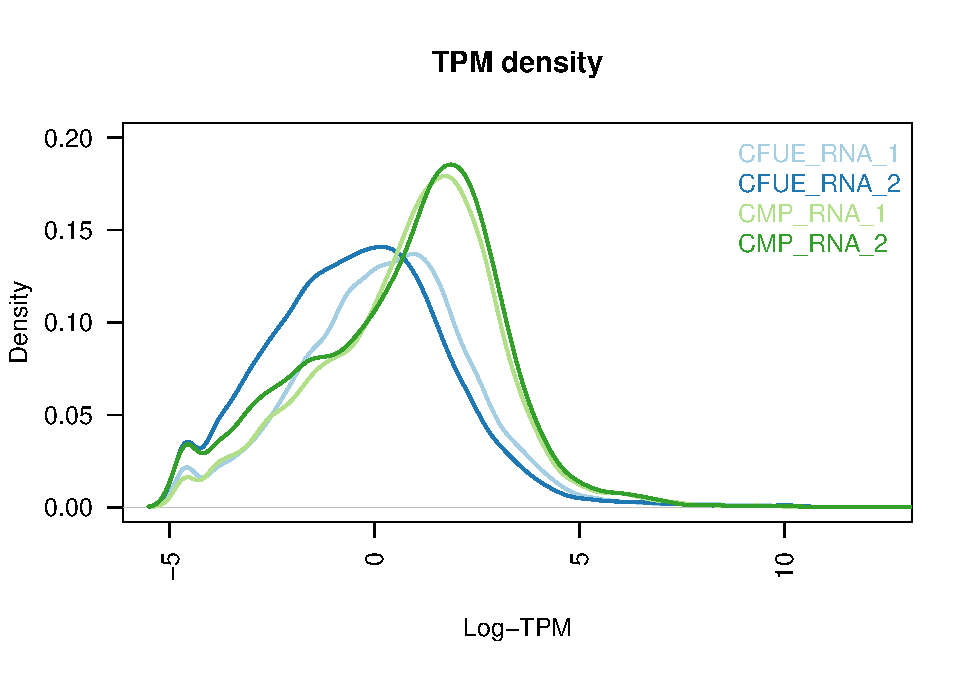
\includegraphics{RNA_Analysis_23_files/figure-latex/EDA-1.pdf}

\hypertarget{eda---heat-map}{%
\subsection{EDA - Heat map}\label{eda---heat-map}}

Here, we look at the TPM (trascripts per million) for our two cell lines
(2 replicates each), and we pull out the top 100 genes with the highest
variance of expression across samples. Then we plot their normalized
expression levels across the samples using a heat map. We should see
that the replicates within each cell line should have a more similar
expression pattern than across cell lines.

\begin{Shaded}
\begin{Highlighting}[]
\FunctionTok{library}\NormalTok{(pheatmap)}
\end{Highlighting}
\end{Shaded}

\begin{verbatim}
## Warning: package 'pheatmap' was built under R version 4.3.3
\end{verbatim}

\begin{Shaded}
\begin{Highlighting}[]
\CommentTok{\#compute the variance of each gene across samples}
\NormalTok{variances }\OtherTok{\textless{}{-}} \FunctionTok{apply}\NormalTok{(tpm, }\DecValTok{1}\NormalTok{, var)}

\NormalTok{selectedGenes }\OtherTok{\textless{}{-}} \FunctionTok{order}\NormalTok{(variances, }\AttributeTok{decreasing =} \ConstantTok{TRUE}\NormalTok{)[}\DecValTok{1}\SpecialCharTok{:}\DecValTok{100}\NormalTok{]}
\FunctionTok{pheatmap}\NormalTok{(tpm[selectedGenes,], }\AttributeTok{scale =} \StringTok{\textquotesingle{}row\textquotesingle{}}\NormalTok{, }\AttributeTok{show\_rownames =} \ConstantTok{FALSE}\NormalTok{)}
\end{Highlighting}
\end{Shaded}

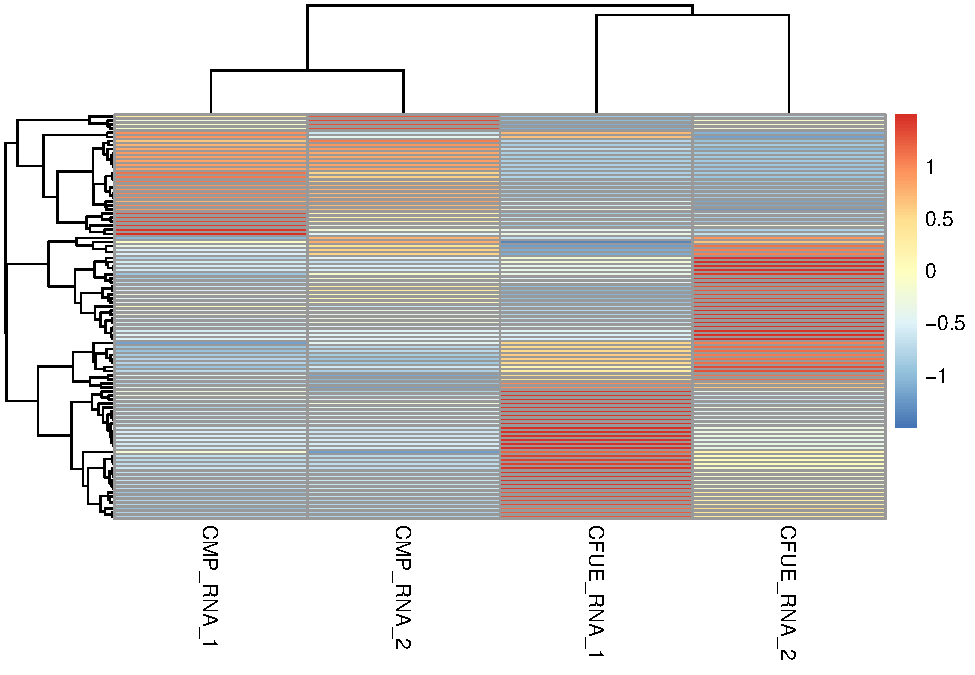
\includegraphics{RNA_Analysis_23_files/figure-latex/heat map-1.pdf}

\hypertarget{eda---pca}{%
\subsection{EDA - PCA}\label{eda---pca}}

\ldots{}

\begin{Shaded}
\begin{Highlighting}[]
\FunctionTok{library}\NormalTok{(stats)}
\FunctionTok{library}\NormalTok{(ggplot2)}
\end{Highlighting}
\end{Shaded}

\begin{verbatim}
## Warning: package 'ggplot2' was built under R version 4.3.3
\end{verbatim}

\begin{Shaded}
\begin{Highlighting}[]
\FunctionTok{library}\NormalTok{(ellipse)}
\end{Highlighting}
\end{Shaded}

\begin{verbatim}
## 
## Attaching package: 'ellipse'
\end{verbatim}

\begin{verbatim}
## The following object is masked from 'package:graphics':
## 
##     pairs
\end{verbatim}

\begin{Shaded}
\begin{Highlighting}[]
\NormalTok{M }\OtherTok{\textless{}{-}} \FunctionTok{t}\NormalTok{(tpm[selectedGenes,])}
\NormalTok{M }\OtherTok{\textless{}{-}} \FunctionTok{log2}\NormalTok{(M }\SpecialCharTok{+} \DecValTok{1}\NormalTok{)}
\NormalTok{pcaResults }\OtherTok{\textless{}{-}} \FunctionTok{prcomp}\NormalTok{(M)}

\CommentTok{\# Extract principal components from the PCA results}
\NormalTok{pc }\OtherTok{\textless{}{-}} \FunctionTok{data.frame}\NormalTok{(}\AttributeTok{PC1 =}\NormalTok{ pcaResults}\SpecialCharTok{$}\NormalTok{x[,}\DecValTok{1}\NormalTok{], }\AttributeTok{PC2 =}\NormalTok{ pcaResults}\SpecialCharTok{$}\NormalTok{x[,}\DecValTok{2}\NormalTok{])}

\CommentTok{\# Add sample metadata from colData}
\NormalTok{pc }\OtherTok{\textless{}{-}} \FunctionTok{cbind}\NormalTok{(pc, colData)}

\CommentTok{\# Plot PCA results using ggplot2}
\FunctionTok{ggplot}\NormalTok{(pc, }\FunctionTok{aes}\NormalTok{(}\AttributeTok{x =}\NormalTok{ PC1, }\AttributeTok{y =}\NormalTok{ PC2, }\AttributeTok{color =}\NormalTok{ group)) }\SpecialCharTok{+}
  \FunctionTok{geom\_point}\NormalTok{() }\SpecialCharTok{+}
  \FunctionTok{labs}\NormalTok{(}\AttributeTok{title =} \StringTok{"PCA Plot"}\NormalTok{, }\AttributeTok{x =} \StringTok{"PC1"}\NormalTok{, }\AttributeTok{y =} \StringTok{"PC2"}\NormalTok{)}
\end{Highlighting}
\end{Shaded}

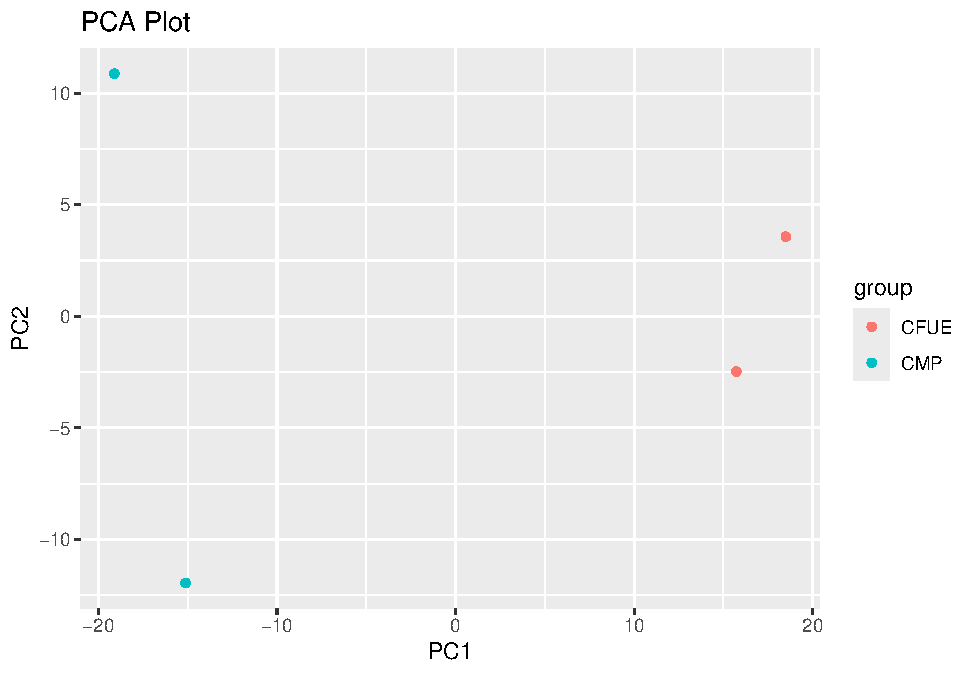
\includegraphics{RNA_Analysis_23_files/figure-latex/PCA-1.pdf}

\begin{Shaded}
\begin{Highlighting}[]
\FunctionTok{summary}\NormalTok{(pcaResults)}
\end{Highlighting}
\end{Shaded}

\begin{verbatim}
## Importance of components:
##                            PC1    PC2     PC3       PC4
## Standard deviation     19.8561 9.6610 5.65563 7.318e-15
## Proportion of Variance  0.7588 0.1796 0.06156 0.000e+00
## Cumulative Proportion   0.7588 0.9384 1.00000 1.000e+00
\end{verbatim}

\hypertarget{correlation-plots}{%
\subsection{Correlation plots}\label{correlation-plots}}

\begin{Shaded}
\begin{Highlighting}[]
\FunctionTok{library}\NormalTok{(corrplot)}
\end{Highlighting}
\end{Shaded}

\begin{verbatim}
## corrplot 0.92 loaded
\end{verbatim}

\begin{Shaded}
\begin{Highlighting}[]
\NormalTok{correlationMatrix }\OtherTok{\textless{}{-}} \FunctionTok{cor}\NormalTok{(tpm)}
\FunctionTok{corrplot}\NormalTok{(correlationMatrix, }\AttributeTok{order =} \StringTok{\textquotesingle{}hclust\textquotesingle{}}\NormalTok{, }
         \AttributeTok{addrect =} \DecValTok{2}\NormalTok{, }\AttributeTok{addCoef.col =} \StringTok{\textquotesingle{}white\textquotesingle{}}\NormalTok{, }
         \AttributeTok{number.cex =} \FloatTok{0.7}\NormalTok{) }
\end{Highlighting}
\end{Shaded}

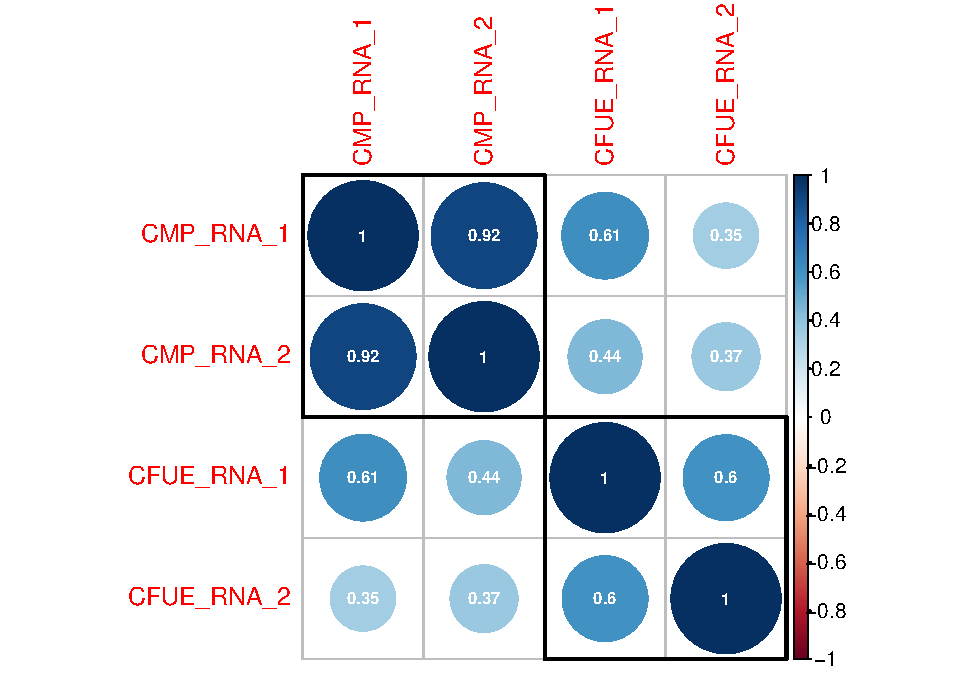
\includegraphics{RNA_Analysis_23_files/figure-latex/cor plots-1.pdf}

\hypertarget{differential-expression-analysis}{%
\section{Differential Expression
Analysis}\label{differential-expression-analysis}}

\hypertarget{preprocessing}{%
\subsection{Preprocessing}\label{preprocessing}}

\begin{Shaded}
\begin{Highlighting}[]
\CommentTok{\#Get counts data}
\CommentTok{\# Add prefixes to the tpm columns in each dataframe}
\NormalTok{CFUE\_RNA\_1\_counts }\OtherTok{\textless{}{-}}\NormalTok{ CFUE\_RNA\_1 }\SpecialCharTok{\%\textgreater{}\%} \FunctionTok{select}\NormalTok{(gene\_id, }\AttributeTok{CFUE\_RNA\_1\_counts =}\NormalTok{ expected\_count)}
\NormalTok{CFUE\_RNA\_2\_counts }\OtherTok{\textless{}{-}}\NormalTok{ CFUE\_RNA\_2 }\SpecialCharTok{\%\textgreater{}\%} \FunctionTok{select}\NormalTok{(gene\_id, }\AttributeTok{CFUE\_RNA\_2\_counts =}\NormalTok{ expected\_count)}
\NormalTok{CMP\_RNA\_1\_counts }\OtherTok{\textless{}{-}}\NormalTok{ CMP\_RNA\_1 }\SpecialCharTok{\%\textgreater{}\%} \FunctionTok{select}\NormalTok{(gene\_id, }\AttributeTok{CMP\_RNA\_1\_counts =}\NormalTok{ expected\_count)}
\NormalTok{CMP\_RNA\_2\_counts }\OtherTok{\textless{}{-}}\NormalTok{ CMP\_RNA\_2 }\SpecialCharTok{\%\textgreater{}\%} \FunctionTok{select}\NormalTok{(gene\_id, }\AttributeTok{CMP\_RNA\_2\_counts =}\NormalTok{ expected\_count)}

\CommentTok{\# Join the dataframes together on gene\_id}
\NormalTok{countData }\OtherTok{\textless{}{-}} \FunctionTok{inner\_join}\NormalTok{(CFUE\_RNA\_1\_counts, CFUE\_RNA\_2\_counts, }\AttributeTok{by =} \StringTok{"gene\_id"}\NormalTok{) }\SpecialCharTok{\%\textgreater{}\%}
       \FunctionTok{inner\_join}\NormalTok{(CMP\_RNA\_1\_counts, }\AttributeTok{by =} \StringTok{"gene\_id"}\NormalTok{) }\SpecialCharTok{\%\textgreater{}\%}
       \FunctionTok{inner\_join}\NormalTok{(CMP\_RNA\_2\_counts, }\AttributeTok{by =} \StringTok{"gene\_id"}\NormalTok{) }

\FunctionTok{rm}\NormalTok{(CFUE\_RNA\_1\_counts, CFUE\_RNA\_2\_counts, CMP\_RNA\_1\_counts, CMP\_RNA\_2\_counts)}

\NormalTok{countData }\OtherTok{\textless{}{-}}\NormalTok{ countData }\SpecialCharTok{\%\textgreater{}\%}
  \FunctionTok{rename\_at}\NormalTok{(}\FunctionTok{vars}\NormalTok{(}\DecValTok{2}\SpecialCharTok{:}\DecValTok{5}\NormalTok{), }\SpecialCharTok{\textasciitilde{}} \FunctionTok{sub}\NormalTok{(}\StringTok{"\_counts$"}\NormalTok{, }\StringTok{""}\NormalTok{, .))}

\NormalTok{countData }\OtherTok{\textless{}{-}} \FunctionTok{mutate\_if}\NormalTok{(countData, is.numeric, round)}

\CommentTok{\# Set \textquotesingle{}column\_name\textquotesingle{} as row names}
\FunctionTok{rownames}\NormalTok{(countData) }\OtherTok{\textless{}{-}}\NormalTok{ countData}\SpecialCharTok{$}\NormalTok{gene\_id}

\CommentTok{\# Remove \textquotesingle{}column\_name\textquotesingle{} from dataframe (optional)}
\NormalTok{countData }\OtherTok{\textless{}{-}}\NormalTok{ countData[, }\SpecialCharTok{{-}}\FunctionTok{which}\NormalTok{(}\FunctionTok{names}\NormalTok{(countData) }\SpecialCharTok{==} \StringTok{\textquotesingle{}gene\_id\textquotesingle{}}\NormalTok{)]}

\CommentTok{\#Create a colData matrix}
\NormalTok{colData }\OtherTok{=} \FunctionTok{data.frame}\NormalTok{(}
  \AttributeTok{source\_name =} \FunctionTok{c}\NormalTok{(}\StringTok{\textquotesingle{}CMP\_RNA\_1\textquotesingle{}}\NormalTok{,}\StringTok{\textquotesingle{}CMP\_RNA\_2\textquotesingle{}}\NormalTok{,}\StringTok{\textquotesingle{}CFUE\_RNA\_1\textquotesingle{}}\NormalTok{,}\StringTok{\textquotesingle{}CFUE\_RNA\_2\textquotesingle{}}\NormalTok{),}
  \AttributeTok{group =} \FunctionTok{c}\NormalTok{(}\StringTok{\textquotesingle{}CMP\textquotesingle{}}\NormalTok{, }\StringTok{\textquotesingle{}CMP\textquotesingle{}}\NormalTok{, }\StringTok{\textquotesingle{}CFUE\textquotesingle{}}\NormalTok{, }\StringTok{\textquotesingle{}CFUE\textquotesingle{}}\NormalTok{)}
\NormalTok{  )}
\NormalTok{colData}\SpecialCharTok{$}\NormalTok{group }\OtherTok{=} \FunctionTok{as.factor}\NormalTok{(colData}\SpecialCharTok{$}\NormalTok{group)}
\NormalTok{designFormula }\OtherTok{\textless{}{-}} \StringTok{"\textasciitilde{} group"}
\end{Highlighting}
\end{Shaded}

\hypertarget{deseq2}{%
\subsection{DESeq2}\label{deseq2}}

\begin{Shaded}
\begin{Highlighting}[]
\FunctionTok{library}\NormalTok{(DESeq2)}
\end{Highlighting}
\end{Shaded}

\begin{verbatim}
## Warning: package 'DESeq2' was built under R version 4.3.3
\end{verbatim}

\begin{verbatim}
## Loading required package: S4Vectors
\end{verbatim}

\begin{verbatim}
## Loading required package: stats4
\end{verbatim}

\begin{verbatim}
## Loading required package: BiocGenerics
\end{verbatim}

\begin{verbatim}
## 
## Attaching package: 'BiocGenerics'
\end{verbatim}

\begin{verbatim}
## The following objects are masked from 'package:dplyr':
## 
##     combine, intersect, setdiff, union
\end{verbatim}

\begin{verbatim}
## The following objects are masked from 'package:stats':
## 
##     IQR, mad, sd, var, xtabs
\end{verbatim}

\begin{verbatim}
## The following objects are masked from 'package:base':
## 
##     anyDuplicated, aperm, append, as.data.frame, basename, cbind,
##     colnames, dirname, do.call, duplicated, eval, evalq, Filter, Find,
##     get, grep, grepl, intersect, is.unsorted, lapply, Map, mapply,
##     match, mget, order, paste, pmax, pmax.int, pmin, pmin.int,
##     Position, rank, rbind, Reduce, rownames, sapply, setdiff, sort,
##     table, tapply, union, unique, unsplit, which.max, which.min
\end{verbatim}

\begin{verbatim}
## 
## Attaching package: 'S4Vectors'
\end{verbatim}

\begin{verbatim}
## The following objects are masked from 'package:dplyr':
## 
##     first, rename
\end{verbatim}

\begin{verbatim}
## The following object is masked from 'package:utils':
## 
##     findMatches
\end{verbatim}

\begin{verbatim}
## The following objects are masked from 'package:base':
## 
##     expand.grid, I, unname
\end{verbatim}

\begin{verbatim}
## Loading required package: IRanges
\end{verbatim}

\begin{verbatim}
## 
## Attaching package: 'IRanges'
\end{verbatim}

\begin{verbatim}
## The following objects are masked from 'package:dplyr':
## 
##     collapse, desc, slice
\end{verbatim}

\begin{verbatim}
## The following object is masked from 'package:grDevices':
## 
##     windows
\end{verbatim}

\begin{verbatim}
## Loading required package: GenomicRanges
\end{verbatim}

\begin{verbatim}
## Loading required package: GenomeInfoDb
\end{verbatim}

\begin{verbatim}
## Warning: package 'GenomeInfoDb' was built under R version 4.3.3
\end{verbatim}

\begin{verbatim}
## Loading required package: SummarizedExperiment
\end{verbatim}

\begin{verbatim}
## Loading required package: MatrixGenerics
\end{verbatim}

\begin{verbatim}
## Loading required package: matrixStats
\end{verbatim}

\begin{verbatim}
## 
## Attaching package: 'matrixStats'
\end{verbatim}

\begin{verbatim}
## The following object is masked from 'package:dplyr':
## 
##     count
\end{verbatim}

\begin{verbatim}
## 
## Attaching package: 'MatrixGenerics'
\end{verbatim}

\begin{verbatim}
## The following objects are masked from 'package:matrixStats':
## 
##     colAlls, colAnyNAs, colAnys, colAvgsPerRowSet, colCollapse,
##     colCounts, colCummaxs, colCummins, colCumprods, colCumsums,
##     colDiffs, colIQRDiffs, colIQRs, colLogSumExps, colMadDiffs,
##     colMads, colMaxs, colMeans2, colMedians, colMins, colOrderStats,
##     colProds, colQuantiles, colRanges, colRanks, colSdDiffs, colSds,
##     colSums2, colTabulates, colVarDiffs, colVars, colWeightedMads,
##     colWeightedMeans, colWeightedMedians, colWeightedSds,
##     colWeightedVars, rowAlls, rowAnyNAs, rowAnys, rowAvgsPerColSet,
##     rowCollapse, rowCounts, rowCummaxs, rowCummins, rowCumprods,
##     rowCumsums, rowDiffs, rowIQRDiffs, rowIQRs, rowLogSumExps,
##     rowMadDiffs, rowMads, rowMaxs, rowMeans2, rowMedians, rowMins,
##     rowOrderStats, rowProds, rowQuantiles, rowRanges, rowRanks,
##     rowSdDiffs, rowSds, rowSums2, rowTabulates, rowVarDiffs, rowVars,
##     rowWeightedMads, rowWeightedMeans, rowWeightedMedians,
##     rowWeightedSds, rowWeightedVars
\end{verbatim}

\begin{verbatim}
## Loading required package: Biobase
\end{verbatim}

\begin{verbatim}
## Welcome to Bioconductor
## 
##     Vignettes contain introductory material; view with
##     'browseVignettes()'. To cite Bioconductor, see
##     'citation("Biobase")', and for packages 'citation("pkgname")'.
\end{verbatim}

\begin{verbatim}
## 
## Attaching package: 'Biobase'
\end{verbatim}

\begin{verbatim}
## The following object is masked from 'package:MatrixGenerics':
## 
##     rowMedians
\end{verbatim}

\begin{verbatim}
## The following objects are masked from 'package:matrixStats':
## 
##     anyMissing, rowMedians
\end{verbatim}

\begin{Shaded}
\begin{Highlighting}[]
\CommentTok{\#create a DESeq dataset object from the count matrix and the colData }
\NormalTok{dds }\OtherTok{\textless{}{-}} \FunctionTok{DESeqDataSetFromMatrix}\NormalTok{(}\AttributeTok{countData =}\NormalTok{ countData, }
                              \AttributeTok{colData =}\NormalTok{ colData, }
                              \AttributeTok{design =} \FunctionTok{as.formula}\NormalTok{(designFormula))}
\end{Highlighting}
\end{Shaded}

\begin{verbatim}
## converting counts to integer mode
\end{verbatim}

\begin{Shaded}
\begin{Highlighting}[]
\CommentTok{\#print dds object to see the contents}
\FunctionTok{print}\NormalTok{(dds)}
\end{Highlighting}
\end{Shaded}

\begin{verbatim}
## class: DESeqDataSet 
## dim: 69691 4 
## metadata(1): version
## assays(1): counts
## rownames(69691): 10000 10001 ... gSpikein_ERCC-00171 gSpikein_phiX174
## rowData names(0):
## colnames(4): CFUE_RNA_1 CFUE_RNA_2 CMP_RNA_1 CMP_RNA_2
## colData names(2): source_name group
\end{verbatim}

\begin{Shaded}
\begin{Highlighting}[]
\CommentTok{\#For each gene, we count the total number of reads for that gene in all samples }
\CommentTok{\#and remove those that don\textquotesingle{}t have at least 1 read. }
\NormalTok{dds }\OtherTok{\textless{}{-}}\NormalTok{ dds[ }\FunctionTok{rowSums}\NormalTok{(DESeq2}\SpecialCharTok{::}\FunctionTok{counts}\NormalTok{(dds)) }\SpecialCharTok{\textgreater{}} \DecValTok{1}\NormalTok{, ]}

\NormalTok{dds }\OtherTok{\textless{}{-}} \FunctionTok{DESeq}\NormalTok{(dds)}
\end{Highlighting}
\end{Shaded}

\begin{verbatim}
## estimating size factors
\end{verbatim}

\begin{verbatim}
## estimating dispersions
\end{verbatim}

\begin{verbatim}
## gene-wise dispersion estimates
\end{verbatim}

\begin{verbatim}
## mean-dispersion relationship
\end{verbatim}

\begin{verbatim}
## final dispersion estimates
\end{verbatim}

\begin{verbatim}
## fitting model and testing
\end{verbatim}

\begin{Shaded}
\begin{Highlighting}[]
\CommentTok{\#compute the contrast for the \textquotesingle{}group\textquotesingle{} variable where \textquotesingle{}CTRL\textquotesingle{} }
\CommentTok{\#samples are used as the control group. }
\NormalTok{DEresults }\OtherTok{=} \FunctionTok{results}\NormalTok{(dds, }\AttributeTok{contrast =} \FunctionTok{c}\NormalTok{(}\StringTok{"group"}\NormalTok{, }\StringTok{\textquotesingle{}CMP\textquotesingle{}}\NormalTok{, }\StringTok{\textquotesingle{}CFUE\textquotesingle{}}\NormalTok{))}
\CommentTok{\#sort results by increasing p{-}value}
\NormalTok{DEresults\_print }\OtherTok{\textless{}{-}}\NormalTok{ DEresults[}\FunctionTok{order}\NormalTok{(DEresults}\SpecialCharTok{$}\NormalTok{pvalue)[}\DecValTok{1}\SpecialCharTok{:}\DecValTok{10}\NormalTok{],]}
\FunctionTok{print}\NormalTok{(DEresults)}
\end{Highlighting}
\end{Shaded}

\begin{verbatim}
## log2 fold change (MLE): group CMP vs CFUE 
## Wald test p-value: group CMP vs CFUE 
## DataFrame with 18135 rows and 6 columns
##                         baseMean log2FoldChange     lfcSE       stat
##                        <numeric>      <numeric> <numeric>  <numeric>
## 22050                    5.16515        6.75602  4.804424    1.40621
## 31383                    9.18249        7.58864  4.795805    1.58235
## 46219                    6.20028       -5.21542  4.789963   -1.08882
## ENSMUSG00000000001.4  3656.99476       -1.12957  0.211447   -5.34209
## ENSMUSG00000000028.10 2398.80485        1.06024  0.205558    5.15787
## ...                          ...            ...       ...        ...
## ENSMUSG00000104514.1     5.94361     -0.0717867   3.73001 -0.0192457
## ENSMUSG00000104517.1     9.70745     -5.8571112   3.90893 -1.4983941
## ENSMUSG00000104523.1     2.86953      5.9034231   4.82020  1.2247248
## ENSMUSG00000104524.1    10.23288     -5.9366056   3.84766 -1.5429118
## ENSMUSG00000104525.1    28.70749      1.1467272   2.62809  0.4363354
##                            pvalue        padj
##                         <numeric>   <numeric>
## 22050                 1.59662e-01          NA
## 31383                 1.13570e-01 1.88324e-01
## 46219                 2.76232e-01          NA
## ENSMUSG00000000001.4  9.18807e-08 5.19290e-07
## ENSMUSG00000000028.10 2.49779e-07 1.33909e-06
## ...                           ...         ...
## ENSMUSG00000104514.1     0.984645          NA
## ENSMUSG00000104517.1     0.134031    0.214097
## ENSMUSG00000104523.1     0.220679          NA
## ENSMUSG00000104524.1     0.122852    0.200183
## ENSMUSG00000104525.1     0.662593    0.749143
\end{verbatim}

\hypertarget{diagnostic-plots}{%
\subsection{Diagnostic plots}\label{diagnostic-plots}}

MA plot: Note that most points fall on the horizontal zero line, which
means most genes are not differentially expressed.

P-value plot: It is also important to observe the distribution of raw
p-values. We expect to see a peak around low p-values and a uniform
distribution at P-values above 0.1. Otherwise, adjustment for multiple
testing does not work and the results are not meaningful.

\begin{Shaded}
\begin{Highlighting}[]
\CommentTok{\#MA plot}
\NormalTok{DESeq2}\SpecialCharTok{::}\FunctionTok{plotMA}\NormalTok{(}\AttributeTok{object =}\NormalTok{ dds, }\AttributeTok{ylim =} \FunctionTok{c}\NormalTok{(}\SpecialCharTok{{-}}\DecValTok{5}\NormalTok{, }\DecValTok{5}\NormalTok{))}
\end{Highlighting}
\end{Shaded}

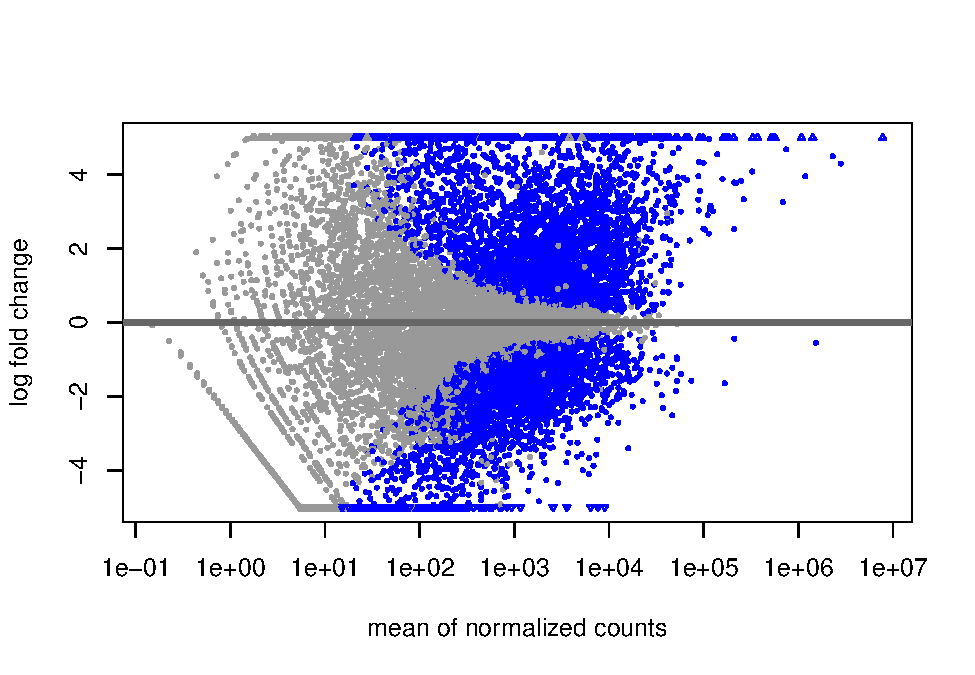
\includegraphics{RNA_Analysis_23_files/figure-latex/diag plots-1.pdf}

\begin{Shaded}
\begin{Highlighting}[]
\CommentTok{\#Pvalue plot}
\FunctionTok{library}\NormalTok{(ggplot2)}
\FunctionTok{ggplot}\NormalTok{(}\AttributeTok{data =} \FunctionTok{as.data.frame}\NormalTok{(DEresults), }\FunctionTok{aes}\NormalTok{(}\AttributeTok{x =}\NormalTok{ pvalue)) }\SpecialCharTok{+} 
  \FunctionTok{geom\_histogram}\NormalTok{(}\AttributeTok{bins =} \DecValTok{100}\NormalTok{)}
\end{Highlighting}
\end{Shaded}

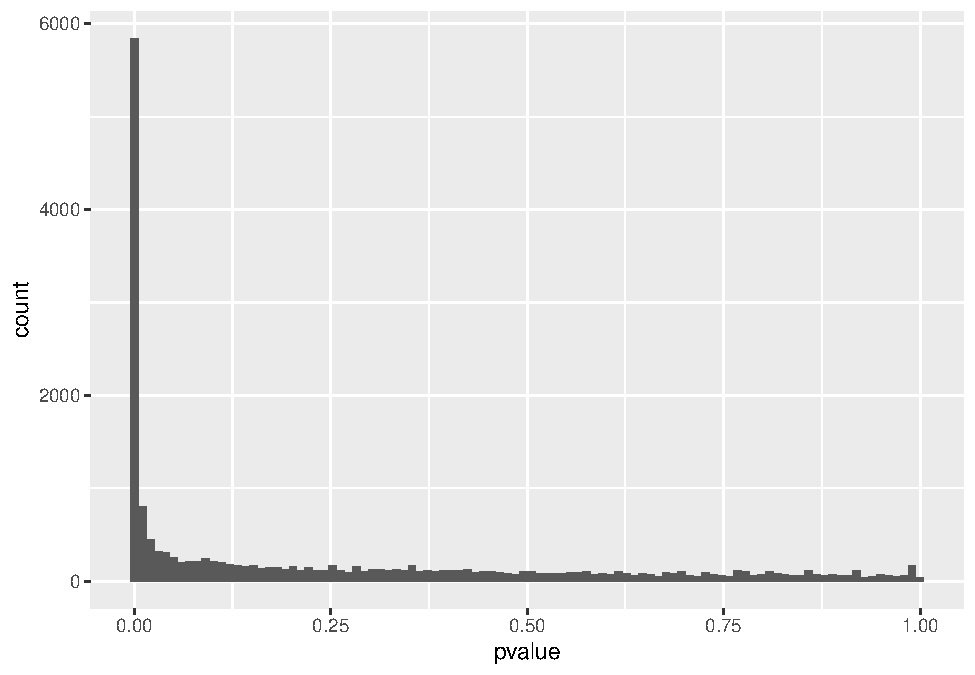
\includegraphics{RNA_Analysis_23_files/figure-latex/diag plots-2.pdf}

\begin{Shaded}
\begin{Highlighting}[]
\CommentTok{\#PCA plot}
\NormalTok{rld }\OtherTok{\textless{}{-}} \FunctionTok{rlog}\NormalTok{(dds)}
\NormalTok{DESeq2}\SpecialCharTok{::}\FunctionTok{plotPCA}\NormalTok{(rld, }\AttributeTok{ntop =} \DecValTok{500}\NormalTok{, }\AttributeTok{intgroup =} \StringTok{\textquotesingle{}group\textquotesingle{}}\NormalTok{) }\SpecialCharTok{+} 
  \FunctionTok{ylim}\NormalTok{(}\SpecialCharTok{{-}}\DecValTok{50}\NormalTok{, }\DecValTok{50}\NormalTok{) }\SpecialCharTok{+} \FunctionTok{theme\_bw}\NormalTok{()}
\end{Highlighting}
\end{Shaded}

\begin{verbatim}
## using ntop=500 top features by variance
\end{verbatim}

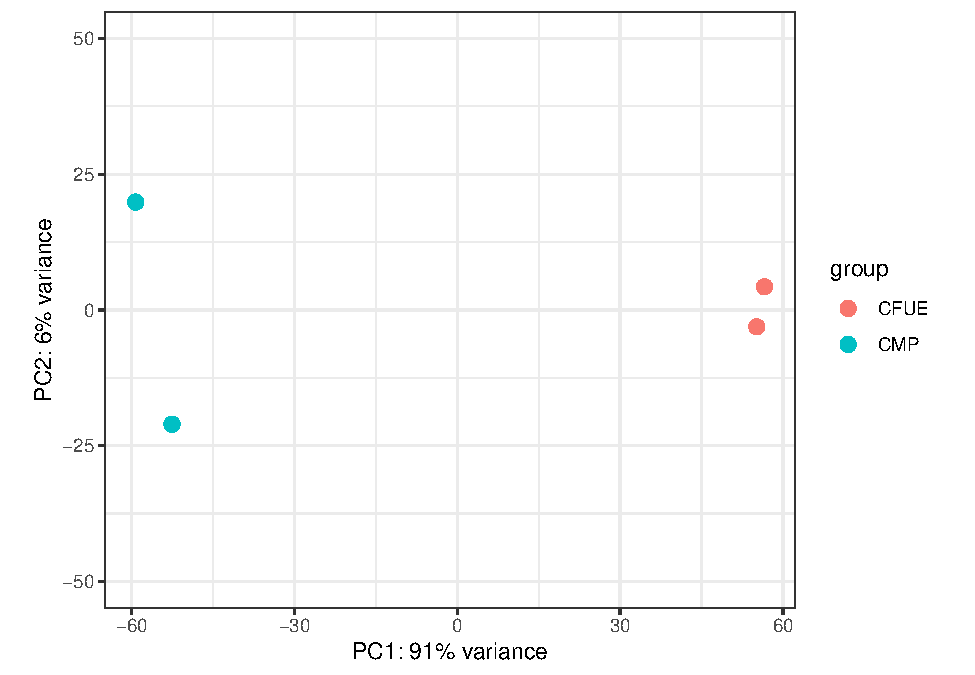
\includegraphics{RNA_Analysis_23_files/figure-latex/diag plots-3.pdf}

\begin{Shaded}
\begin{Highlighting}[]
\CommentTok{\#RLE Plot}
\FunctionTok{library}\NormalTok{(EDASeq)}
\end{Highlighting}
\end{Shaded}

\begin{verbatim}
## Loading required package: ShortRead
\end{verbatim}

\begin{verbatim}
## Loading required package: BiocParallel
\end{verbatim}

\begin{verbatim}
## Loading required package: Biostrings
\end{verbatim}

\begin{verbatim}
## Warning: package 'Biostrings' was built under R version 4.3.3
\end{verbatim}

\begin{verbatim}
## Loading required package: XVector
\end{verbatim}

\begin{verbatim}
## 
## Attaching package: 'Biostrings'
\end{verbatim}

\begin{verbatim}
## The following object is masked from 'package:base':
## 
##     strsplit
\end{verbatim}

\begin{verbatim}
## Loading required package: Rsamtools
\end{verbatim}

\begin{verbatim}
## Loading required package: GenomicAlignments
\end{verbatim}

\begin{verbatim}
## 
## Attaching package: 'GenomicAlignments'
\end{verbatim}

\begin{verbatim}
## The following object is masked from 'package:dplyr':
## 
##     last
\end{verbatim}

\begin{verbatim}
## 
## Attaching package: 'ShortRead'
\end{verbatim}

\begin{verbatim}
## The following object is masked from 'package:dplyr':
## 
##     id
\end{verbatim}

\begin{Shaded}
\begin{Highlighting}[]
\FunctionTok{par}\NormalTok{(}\AttributeTok{mfrow =} \FunctionTok{c}\NormalTok{(}\DecValTok{1}\NormalTok{, }\DecValTok{1}\NormalTok{))}
\FunctionTok{plotRLE}\NormalTok{(DESeq2}\SpecialCharTok{::}\FunctionTok{counts}\NormalTok{(dds, }\AttributeTok{normalized =} \ConstantTok{TRUE}\NormalTok{), }
        \AttributeTok{outline=}\ConstantTok{FALSE}\NormalTok{, }\AttributeTok{ylim=}\FunctionTok{c}\NormalTok{(}\SpecialCharTok{{-}}\DecValTok{4}\NormalTok{, }\DecValTok{4}\NormalTok{), }
        \AttributeTok{col =} \FunctionTok{as.numeric}\NormalTok{(colData}\SpecialCharTok{$}\NormalTok{group), }
        \AttributeTok{main =} \StringTok{\textquotesingle{}Normalized Counts\textquotesingle{}}\NormalTok{)}
\end{Highlighting}
\end{Shaded}

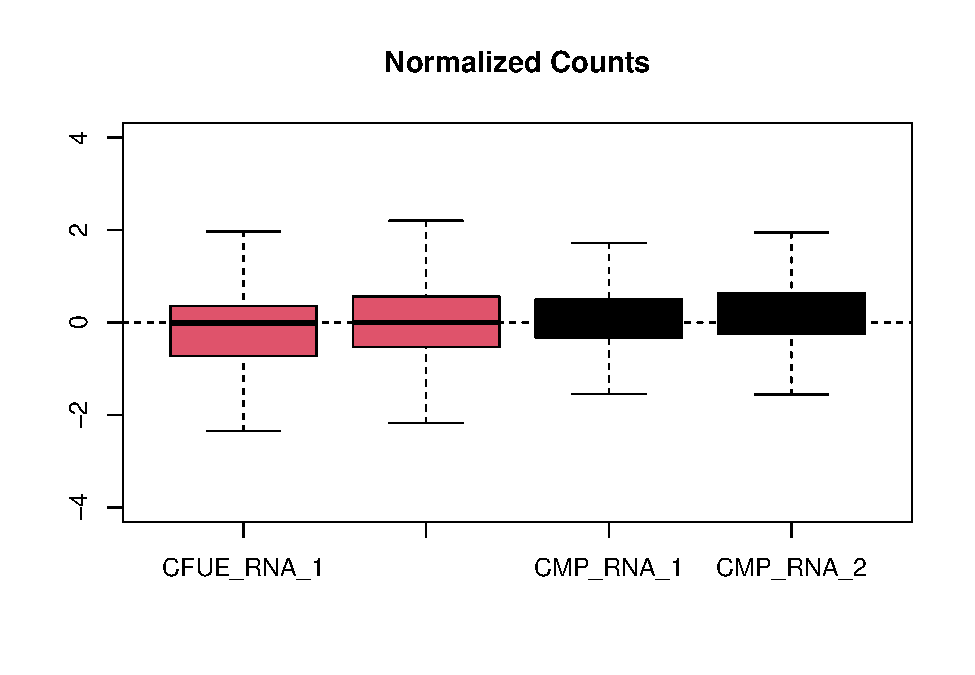
\includegraphics{RNA_Analysis_23_files/figure-latex/diag plots-4.pdf}

\hypertarget{limma-voom}{%
\subsection{Limma-VOOM}\label{limma-voom}}

\begin{Shaded}
\begin{Highlighting}[]
\FunctionTok{library}\NormalTok{(edgeR)}
\end{Highlighting}
\end{Shaded}

\begin{verbatim}
## Loading required package: limma
\end{verbatim}

\begin{verbatim}
## 
## Attaching package: 'limma'
\end{verbatim}

\begin{verbatim}
## The following object is masked from 'package:DESeq2':
## 
##     plotMA
\end{verbatim}

\begin{verbatim}
## The following object is masked from 'package:BiocGenerics':
## 
##     plotMA
\end{verbatim}

\begin{Shaded}
\begin{Highlighting}[]
\CommentTok{\#Create DGEList object}
\NormalTok{d0 }\OtherTok{\textless{}{-}} \FunctionTok{DGEList}\NormalTok{(countData)}

\CommentTok{\#Add normalizing factors}
\NormalTok{d0 }\OtherTok{\textless{}{-}} \FunctionTok{calcNormFactors}\NormalTok{(d0)}

\CommentTok{\#Drop low{-}expressed genes}
\NormalTok{cutoff }\OtherTok{\textless{}{-}} \DecValTok{5}
\NormalTok{drop }\OtherTok{\textless{}{-}} \FunctionTok{which}\NormalTok{(}\FunctionTok{apply}\NormalTok{(}\FunctionTok{cpm}\NormalTok{(d0), }\DecValTok{1}\NormalTok{, max) }\SpecialCharTok{\textless{}}\NormalTok{ cutoff)}
\NormalTok{d }\OtherTok{\textless{}{-}}\NormalTok{ d0[}\SpecialCharTok{{-}}\NormalTok{drop,] }
\FunctionTok{dim}\NormalTok{(d) }\CommentTok{\# number of genes left}
\end{Highlighting}
\end{Shaded}

\begin{verbatim}
## [1] 10461     4
\end{verbatim}

\begin{Shaded}
\begin{Highlighting}[]
\NormalTok{group }\OtherTok{=} \FunctionTok{c}\NormalTok{(}\StringTok{\textquotesingle{}CMP\textquotesingle{}}\NormalTok{, }\StringTok{\textquotesingle{}CMP\textquotesingle{}}\NormalTok{, }\StringTok{\textquotesingle{}CFUE\textquotesingle{}}\NormalTok{, }\StringTok{\textquotesingle{}CFUE\textquotesingle{}}\NormalTok{)}

\NormalTok{mm }\OtherTok{\textless{}{-}} \FunctionTok{model.matrix}\NormalTok{(}\SpecialCharTok{\textasciitilde{}}\NormalTok{group)}
\FunctionTok{colnames}\NormalTok{(mm) }\OtherTok{\textless{}{-}} \FunctionTok{gsub}\NormalTok{(}\StringTok{"group"}\NormalTok{, }\StringTok{""}\NormalTok{, }\FunctionTok{colnames}\NormalTok{(mm))}
\FunctionTok{print}\NormalTok{(mm)}
\end{Highlighting}
\end{Shaded}

\begin{verbatim}
##   (Intercept) CMP
## 1           1   1
## 2           1   1
## 3           1   0
## 4           1   0
## attr(,"assign")
## [1] 0 1
## attr(,"contrasts")
## attr(,"contrasts")$group
## [1] "contr.treatment"
\end{verbatim}

\begin{Shaded}
\begin{Highlighting}[]
\NormalTok{y }\OtherTok{\textless{}{-}} \FunctionTok{voom}\NormalTok{(d, mm, }\AttributeTok{plot =}\NormalTok{ T)}
\end{Highlighting}
\end{Shaded}

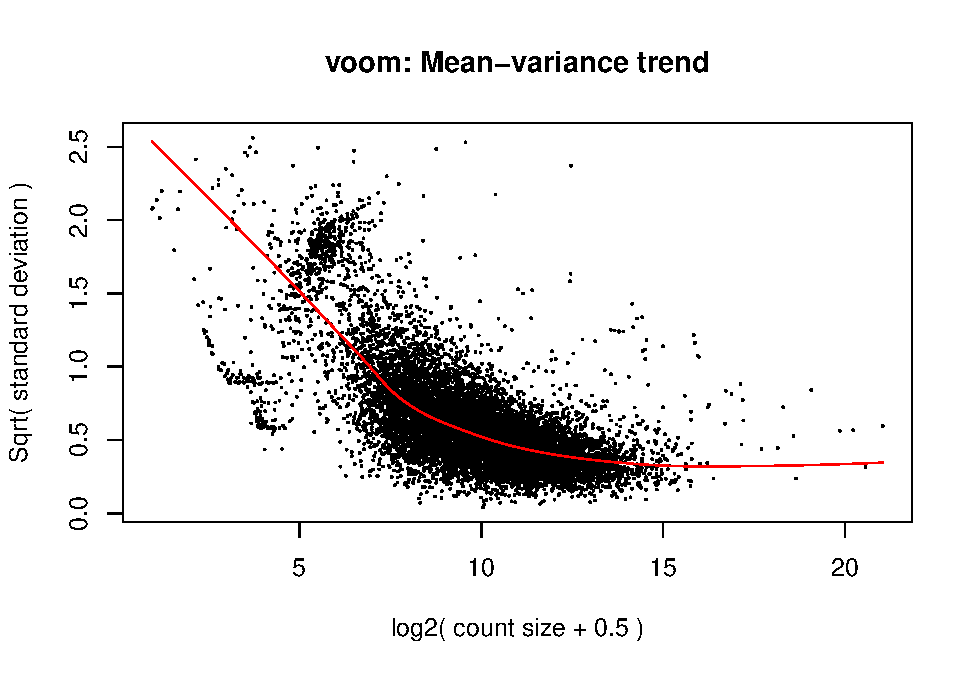
\includegraphics{RNA_Analysis_23_files/figure-latex/limma voom-1.pdf}

\begin{Shaded}
\begin{Highlighting}[]
\NormalTok{fit }\OtherTok{\textless{}{-}} \FunctionTok{lmFit}\NormalTok{(y, mm)}
\FunctionTok{head}\NormalTok{(}\FunctionTok{coef}\NormalTok{(fit))}
\end{Highlighting}
\end{Shaded}

\begin{verbatim}
##                       (Intercept)        CMP
## ENSMUSG00000000001.4     6.766653 -1.2259044
## ENSMUSG00000000028.10    5.085925  0.9858912
## ENSMUSG00000000037.12    2.916188 -1.8348093
## ENSMUSG00000000056.7     5.084557  3.1718361
## ENSMUSG00000000078.6     6.892559 -1.3288026
## ENSMUSG00000000085.12    3.009781  0.3878810
\end{verbatim}

\begin{Shaded}
\begin{Highlighting}[]
\NormalTok{tmp }\OtherTok{\textless{}{-}} \FunctionTok{eBayes}\NormalTok{(fit)}

\NormalTok{top.table }\OtherTok{\textless{}{-}} \FunctionTok{topTable}\NormalTok{(tmp, }\AttributeTok{sort.by =} \StringTok{"P"}\NormalTok{, }\AttributeTok{n =} \ConstantTok{Inf}\NormalTok{)}
\end{Highlighting}
\end{Shaded}

\begin{verbatim}
## Removing intercept from test coefficients
\end{verbatim}

\begin{Shaded}
\begin{Highlighting}[]
\NormalTok{lv\_dif\_ex\_genes }\OtherTok{=} \FunctionTok{rownames}\NormalTok{(}\FunctionTok{head}\NormalTok{(top.table, }\DecValTok{1000}\NormalTok{))}
\end{Highlighting}
\end{Shaded}

\begin{Shaded}
\begin{Highlighting}[]
\FunctionTok{library}\NormalTok{(VennDiagram)}
\end{Highlighting}
\end{Shaded}

\begin{verbatim}
## Warning: package 'VennDiagram' was built under R version 4.3.3
\end{verbatim}

\begin{verbatim}
## Loading required package: grid
\end{verbatim}

\begin{verbatim}
## 
## Attaching package: 'grid'
\end{verbatim}

\begin{verbatim}
## The following object is masked from 'package:Biostrings':
## 
##     pattern
\end{verbatim}

\begin{verbatim}
## Loading required package: futile.logger
\end{verbatim}

\begin{verbatim}
## Warning: package 'futile.logger' was built under R version 4.3.3
\end{verbatim}

\begin{verbatim}
## 
## Attaching package: 'VennDiagram'
\end{verbatim}

\begin{verbatim}
## The following object is masked from 'package:ellipse':
## 
##     ellipse
\end{verbatim}

\begin{Shaded}
\begin{Highlighting}[]
\FunctionTok{library}\NormalTok{(gridExtra)}
\end{Highlighting}
\end{Shaded}

\begin{verbatim}
## 
## Attaching package: 'gridExtra'
\end{verbatim}

\begin{verbatim}
## The following object is masked from 'package:Biobase':
## 
##     combine
\end{verbatim}

\begin{verbatim}
## The following object is masked from 'package:BiocGenerics':
## 
##     combine
\end{verbatim}

\begin{verbatim}
## The following object is masked from 'package:dplyr':
## 
##     combine
\end{verbatim}

\begin{Shaded}
\begin{Highlighting}[]
\CommentTok{\# extract differential expression results}
\NormalTok{DEresults }\OtherTok{\textless{}{-}} \FunctionTok{results}\NormalTok{(dds, }\AttributeTok{contrast =} \FunctionTok{c}\NormalTok{(}\StringTok{\textquotesingle{}group\textquotesingle{}}\NormalTok{, }\StringTok{\textquotesingle{}CMP\textquotesingle{}}\NormalTok{, }\StringTok{\textquotesingle{}CFUE\textquotesingle{}}\NormalTok{))}

\CommentTok{\#remove genes with NA values }
\NormalTok{DE }\OtherTok{\textless{}{-}}\NormalTok{ DEresults[}\SpecialCharTok{!}\FunctionTok{is.na}\NormalTok{(DEresults}\SpecialCharTok{$}\NormalTok{padj),]}
\NormalTok{lowest\_pvalue\_indexes }\OtherTok{\textless{}{-}} \FunctionTok{order}\NormalTok{(DE}\SpecialCharTok{@}\NormalTok{listData}\SpecialCharTok{$}\NormalTok{pvalue)[}\DecValTok{1}\SpecialCharTok{:}\DecValTok{1000}\NormalTok{]}
\NormalTok{DE2\_dif\_ex\_genes }\OtherTok{=}\NormalTok{ DE}\SpecialCharTok{@}\NormalTok{rownames[lowest\_pvalue\_indexes]}

\CommentTok{\# Create a Venn diagram}
\NormalTok{venn.plot }\OtherTok{\textless{}{-}} \FunctionTok{venn.diagram}\NormalTok{(}
  \AttributeTok{x =} \FunctionTok{list}\NormalTok{(lv\_dif\_ex\_genes, DE2\_dif\_ex\_genes),}
  \AttributeTok{category.names =} \FunctionTok{c}\NormalTok{(}\StringTok{"Limma{-}voom"}\NormalTok{ , }\StringTok{"DESEQ2"}\NormalTok{),}
  \AttributeTok{filename =} \StringTok{\textquotesingle{}\#venn\_diagramm.png\textquotesingle{}}\NormalTok{,}
  \AttributeTok{output=}\ConstantTok{TRUE}
\NormalTok{)}
\end{Highlighting}
\end{Shaded}

\hypertarget{go-term-analysis}{%
\subsection{GO term analysis}\label{go-term-analysis}}

Simply run this code on a set of genes that are significantly
upregulated and then same with downregulated

\hypertarget{find-the-upregulated-and-downregulated-gene-descriptions}{%
\paragraph{Find the upregulated and downregulated gene
descriptions}\label{find-the-upregulated-and-downregulated-gene-descriptions}}

\begin{Shaded}
\begin{Highlighting}[]
\FunctionTok{library}\NormalTok{(DESeq2)}
\FunctionTok{library}\NormalTok{(gprofiler2)}
\end{Highlighting}
\end{Shaded}

\begin{verbatim}
## Warning: package 'gprofiler2' was built under R version 4.3.3
\end{verbatim}

\begin{Shaded}
\begin{Highlighting}[]
\FunctionTok{library}\NormalTok{(knitr)}
\CommentTok{\# extract differential expression results}
\NormalTok{DEresults }\OtherTok{\textless{}{-}} \FunctionTok{results}\NormalTok{(dds, }\AttributeTok{contrast =} \FunctionTok{c}\NormalTok{(}\StringTok{\textquotesingle{}group\textquotesingle{}}\NormalTok{, }\StringTok{\textquotesingle{}CMP\textquotesingle{}}\NormalTok{, }\StringTok{\textquotesingle{}CFUE\textquotesingle{}}\NormalTok{))}

\CommentTok{\#remove genes with NA values }
\NormalTok{DE }\OtherTok{\textless{}{-}}\NormalTok{ DEresults[}\SpecialCharTok{!}\FunctionTok{is.na}\NormalTok{(DEresults}\SpecialCharTok{$}\NormalTok{padj),]}
\CommentTok{\#select genes with adjusted p{-}values below 0.1}
\NormalTok{DE }\OtherTok{\textless{}{-}}\NormalTok{ DE[DE}\SpecialCharTok{$}\NormalTok{padj }\SpecialCharTok{\textless{}} \FloatTok{0.1}\NormalTok{,]}
\CommentTok{\#select genes with log2 fold change above 1 (two{-}fold change)}
\NormalTok{up\_reg\_DE }\OtherTok{\textless{}{-}}\NormalTok{ DE[DE}\SpecialCharTok{$}\NormalTok{log2FoldChange }\SpecialCharTok{\textgreater{}} \DecValTok{1}\NormalTok{,]}
\NormalTok{dn\_reg\_DE }\OtherTok{\textless{}{-}}\NormalTok{ DE[DE}\SpecialCharTok{$}\NormalTok{log2FoldChange }\SpecialCharTok{\textless{}} \SpecialCharTok{{-}}\DecValTok{1}\NormalTok{,]}

\CommentTok{\#get the list of upregulated genes of interest}
\NormalTok{up\_reg\_gene\_names }\OtherTok{\textless{}{-}} \FunctionTok{rownames}\NormalTok{(up\_reg\_DE)}
\NormalTok{up\_reg\_gene\_names }\OtherTok{\textless{}{-}} \FunctionTok{sapply}\NormalTok{(}\FunctionTok{strsplit}\NormalTok{(up\_reg\_gene\_names, }\StringTok{"}\SpecialCharTok{\textbackslash{}\textbackslash{}}\StringTok{."}\NormalTok{), }\ControlFlowTok{function}\NormalTok{(x) x[[}\DecValTok{1}\NormalTok{]])}
\NormalTok{up\_reg\_gene\_names }\OtherTok{\textless{}{-}} \FunctionTok{unique}\NormalTok{(up\_reg\_gene\_names)}

\CommentTok{\#get the list of downregulated genes of interest}
\NormalTok{dn\_reg\_gene\_names }\OtherTok{\textless{}{-}} \FunctionTok{rownames}\NormalTok{(dn\_reg\_DE)}
\NormalTok{dn\_reg\_gene\_names }\OtherTok{\textless{}{-}} \FunctionTok{sapply}\NormalTok{(}\FunctionTok{strsplit}\NormalTok{(dn\_reg\_gene\_names, }\StringTok{"}\SpecialCharTok{\textbackslash{}\textbackslash{}}\StringTok{."}\NormalTok{), }\ControlFlowTok{function}\NormalTok{(x) x[[}\DecValTok{1}\NormalTok{]])}
\NormalTok{dn\_reg\_gene\_names }\OtherTok{\textless{}{-}} \FunctionTok{unique}\NormalTok{(dn\_reg\_gene\_names)}

\CommentTok{\#calculate enriched GO terms}
\NormalTok{up\_go\_response }\OtherTok{\textless{}{-}} \FunctionTok{gost}\NormalTok{(}\AttributeTok{query =}\NormalTok{ up\_reg\_gene\_names, }
                     \AttributeTok{organism =} \StringTok{\textquotesingle{}mmusculus\textquotesingle{}}\NormalTok{,}
                  \AttributeTok{sources =} \FunctionTok{c}\NormalTok{(}\StringTok{"GO"}\NormalTok{))}
\NormalTok{dn\_go\_response }\OtherTok{\textless{}{-}} \FunctionTok{gost}\NormalTok{(}\AttributeTok{query =}\NormalTok{ dn\_reg\_gene\_names, }
                     \AttributeTok{organism =} \StringTok{\textquotesingle{}mmusculus\textquotesingle{}}\NormalTok{,}
                  \AttributeTok{sources =} \FunctionTok{c}\NormalTok{(}\StringTok{"GO"}\NormalTok{))}

\CommentTok{\# gostplot(up\_go\_response, capped=FALSE)}
\NormalTok{up\_go\_results }\OtherTok{=}\NormalTok{ up\_go\_response}\SpecialCharTok{$}\NormalTok{result}
\NormalTok{dn\_go\_results }\OtherTok{=}\NormalTok{ dn\_go\_response}\SpecialCharTok{$}\NormalTok{result}
\NormalTok{up\_go\_results }\OtherTok{\textless{}{-}}\NormalTok{ up\_go\_results[}\FunctionTok{order}\NormalTok{(up\_go\_results}\SpecialCharTok{$}\NormalTok{p\_value),]}
\NormalTok{dn\_go\_results }\OtherTok{\textless{}{-}}\NormalTok{ dn\_go\_results[}\FunctionTok{order}\NormalTok{(dn\_go\_results}\SpecialCharTok{$}\NormalTok{p\_value),]}
\CommentTok{\# up\_go\_results \textless{}{-} up\_go\_results[up\_go\_results$intersection\_size \textless{} 100,]}

\FunctionTok{kable}\NormalTok{(up\_go\_results[}\DecValTok{1}\SpecialCharTok{:}\DecValTok{10}\NormalTok{,}\FunctionTok{c}\NormalTok{(}\DecValTok{7}\SpecialCharTok{:}\DecValTok{11}\NormalTok{)])}
\end{Highlighting}
\end{Shaded}

\begin{longtable}[]{@{}
  >{\raggedright\arraybackslash}p{(\columnwidth - 10\tabcolsep) * \real{0.0588}}
  >{\raggedleft\arraybackslash}p{(\columnwidth - 10\tabcolsep) * \real{0.1176}}
  >{\raggedleft\arraybackslash}p{(\columnwidth - 10\tabcolsep) * \real{0.1176}}
  >{\raggedright\arraybackslash}p{(\columnwidth - 10\tabcolsep) * \real{0.1294}}
  >{\raggedright\arraybackslash}p{(\columnwidth - 10\tabcolsep) * \real{0.0824}}
  >{\raggedright\arraybackslash}p{(\columnwidth - 10\tabcolsep) * \real{0.4941}}@{}}
\toprule\noalign{}
\begin{minipage}[b]{\linewidth}\raggedright
\end{minipage} & \begin{minipage}[b]{\linewidth}\raggedleft
precision
\end{minipage} & \begin{minipage}[b]{\linewidth}\raggedleft
recall
\end{minipage} & \begin{minipage}[b]{\linewidth}\raggedright
term\_id
\end{minipage} & \begin{minipage}[b]{\linewidth}\raggedright
source
\end{minipage} & \begin{minipage}[b]{\linewidth}\raggedright
term\_name
\end{minipage} \\
\midrule\noalign{}
\endhead
\bottomrule\noalign{}
\endlastfoot
864 & 0.6466780 & 0.1641726 & \url{GO:0005737} & \url{GO:CC} &
cytoplasm \\
1025 & 0.6250000 & 0.1720841 & \url{GO:0005515} & \url{GO:MF} & protein
binding \\
865 & 0.8293015 & 0.1397887 & \url{GO:0005622} & \url{GO:CC} &
intracellular anatomical structure \\
866 & 0.9550256 & 0.1237364 & \url{GO:0110165} & \url{GO:CC} & cellular
anatomical entity \\
867 & 0.7570698 & 0.1403132 & \url{GO:0043229} & \url{GO:CC} &
intracellular organelle \\
868 & 0.7642249 & 0.1387222 & \url{GO:0043226} & \url{GO:CC} &
organelle \\
1026 & 0.8121528 & 0.1428135 & \url{GO:0005488} & \url{GO:MF} &
binding \\
1 & 0.4013135 & 0.1762028 & \url{GO:0048518} & \url{GO:BP} & positive
regulation of biological process \\
869 & 0.7001704 & 0.1423623 & \url{GO:0043231} & \url{GO:CC} &
intracellular membrane-bounded organelle \\
870 & 0.7148211 & 0.1404848 & \url{GO:0043227} & \url{GO:CC} &
membrane-bounded organelle \\
\end{longtable}

\begin{Shaded}
\begin{Highlighting}[]
\FunctionTok{kable}\NormalTok{(dn\_go\_results[}\DecValTok{1}\SpecialCharTok{:}\DecValTok{10}\NormalTok{,}\FunctionTok{c}\NormalTok{(}\DecValTok{7}\SpecialCharTok{:}\DecValTok{11}\NormalTok{)])}
\end{Highlighting}
\end{Shaded}

\begin{longtable}[]{@{}
  >{\raggedright\arraybackslash}p{(\columnwidth - 10\tabcolsep) * \real{0.0444}}
  >{\raggedleft\arraybackslash}p{(\columnwidth - 10\tabcolsep) * \real{0.1111}}
  >{\raggedleft\arraybackslash}p{(\columnwidth - 10\tabcolsep) * \real{0.1111}}
  >{\raggedright\arraybackslash}p{(\columnwidth - 10\tabcolsep) * \real{0.1222}}
  >{\raggedright\arraybackslash}p{(\columnwidth - 10\tabcolsep) * \real{0.0778}}
  >{\raggedright\arraybackslash}p{(\columnwidth - 10\tabcolsep) * \real{0.5333}}@{}}
\toprule\noalign{}
\begin{minipage}[b]{\linewidth}\raggedright
\end{minipage} & \begin{minipage}[b]{\linewidth}\raggedleft
precision
\end{minipage} & \begin{minipage}[b]{\linewidth}\raggedleft
recall
\end{minipage} & \begin{minipage}[b]{\linewidth}\raggedright
term\_id
\end{minipage} & \begin{minipage}[b]{\linewidth}\raggedright
source
\end{minipage} & \begin{minipage}[b]{\linewidth}\raggedright
term\_name
\end{minipage} \\
\midrule\noalign{}
\endhead
\bottomrule\noalign{}
\endlastfoot
569 & 0.7038184 & 0.1769743 & \url{GO:0005737} & \url{GO:CC} &
cytoplasm \\
570 & 0.8654971 & 0.1444980 & \url{GO:0005622} & \url{GO:CC} &
intracellular anatomical structure \\
571 & 0.7997936 & 0.1437937 & \url{GO:0043226} & \url{GO:CC} &
organelle \\
572 & 0.7884417 & 0.1447335 & \url{GO:0043229} & \url{GO:CC} &
intracellular organelle \\
573 & 0.7481940 & 0.1456408 & \url{GO:0043227} & \url{GO:CC} &
membrane-bounded organelle \\
574 & 0.7230822 & 0.1456183 & \url{GO:0043231} & \url{GO:CC} &
intracellular membrane-bounded organelle \\
1 & 0.3296590 & 0.2029692 & \url{GO:0044271} & \url{GO:BP} & cellular
nitrogen compound biosynthetic process \\
2 & 0.0657940 & 0.5950156 & \url{GO:0042254} & \url{GO:BP} & ribosome
biogenesis \\
575 & 0.2948056 & 0.2087698 & \url{GO:0005829} & \url{GO:CC} &
cytosol \\
576 & 0.9552804 & 0.1225886 & \url{GO:0110165} & \url{GO:CC} & cellular
anatomical entity \\
\end{longtable}

\begin{Shaded}
\begin{Highlighting}[]
\CommentTok{\# gostplot(up\_go\_response, capped = FALSE)}
\CommentTok{\# gostplot(dn\_go\_response, capped = FALSE)}
\end{Highlighting}
\end{Shaded}


\end{document}
